% Original Author: GitHub @leowrs (https://github.com/leowrs)
\documentclass{article}
\usepackage[UTF8]{ctex}  % 支持中文
\usepackage{array}       % 改进表格支持
\usepackage{amsmath}     % 数学公式支持
\usepackage{listings}    % 代码支持
\usepackage{graphicx}    % 图片支持
\usepackage{float}       % 强制图片位置

\begin{document}

\begin{center}
\Large\textbf{Summer School: Introduction to Wireless Communication Systems}\\[0.5em]
\Large\textbf{Tutorial 2}
\end{center}

\begin{center}
\begin{tabular}{|l|l|}
\hline
Student's Chinese Name & @leowrs \\
\hline
Student's ID\# & — \\
\hline
\end{tabular}
\end{center}

\vspace{1em}

\section*{Q1.1. What happens to the bits after modulation?}

原始比特是取值为 \{0, 1\} 的二进制数，通过 MATLAB 代码 \texttt{bpsk\_sig = -2*(bits-0.5)} 进行 BPSK 调制后，比特被映射为两种符号：

\begin{itemize}
    \item 当输入比特为 0 时，调制后的符号为 $-2 \times (0-0.5) = 1$；
    \item 当输入比特为 1 时，调制后的符号为 $-2 \times (1-0.5) = -1$。
\end{itemize}

即二进制比特被转换为幅度相同、相位相反（1 对应 0 弧度，-1 对应 $\pi$ 弧度）的两个符号，实现了二进制信息到相位调制符号的转换。

\section*{Q1.2. Plot the first 10 bits of the received binary data using the MATLAB code below.}

\begin{figure}[H]
    \centering
    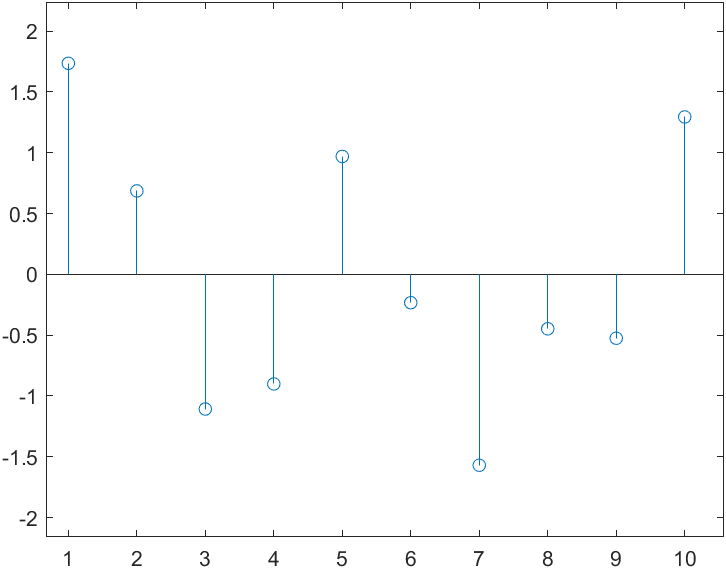
\includegraphics[width=0.8\textwidth]{Tutorial2_1.png}
    \caption{前10个接收比特的图形}
    \label{fig:received_bits}
\end{figure}

\section*{Q1.3. Plot the BER as a function of SNR for SNR=[0: 2: 10] dB using the MATLAB code below. Add axes labels and title to the figure.}

\begin{figure}[H]
    \centering
    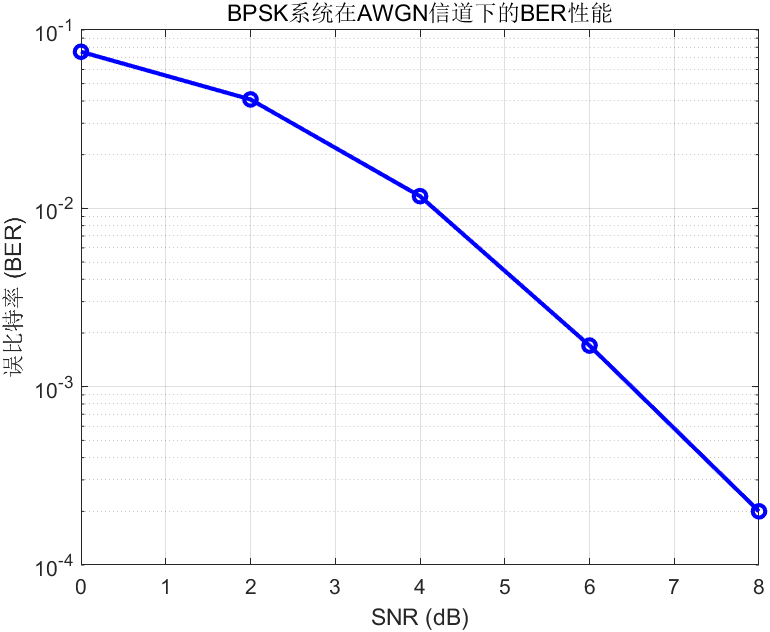
\includegraphics[width=0.8\textwidth]{Tutorial2_2.png}
    \caption{BER vs SNR的图形}
    \label{fig:ber_vs_snr}
\end{figure}

\section*{Q1.4. What do you notice with the BER vs SNR plot? Explain why.}

\textbf{观察：}随着 SNR 的增大，BER 逐渐降低。

\textbf{解释：}SNR 表示信号功率与噪声功率的比值，SNR 越高，信号相对于噪声越强。BPSK 解调通过判断接收符号是否小于 0 来恢复比特（小于 0 判为 1，否则判为 0）。当 SNR 较高时，噪声影响较弱，接收符号很少跨越判决阈值（0），错误比特数少，BER 低；当 SNR 降低时，噪声干扰增强，更多符号被误判，导致 BER 升高。

\end{document}